% The lethal trifecta for Ch27 ("Security: The Adversarial-Input Layer").
% Standalone TikZ; compiled by `book-scaffold build-figures` via pdflatex -> pdftocairo -> SVG.
% Three legs (private-data access, untrusted content, external-communication path) converge on
% catastrophic exfiltration ONLY when all three are present; each robust defense cuts one leg.
% Coinage attributed to Simon Willison (a practitioner framing) — attribution carried in the caption.
\documentclass[tikz,border=4mm]{standalone}
\usepackage{tikz}
\usetikzlibrary{positioning, arrows.meta, calc}

\begin{document}
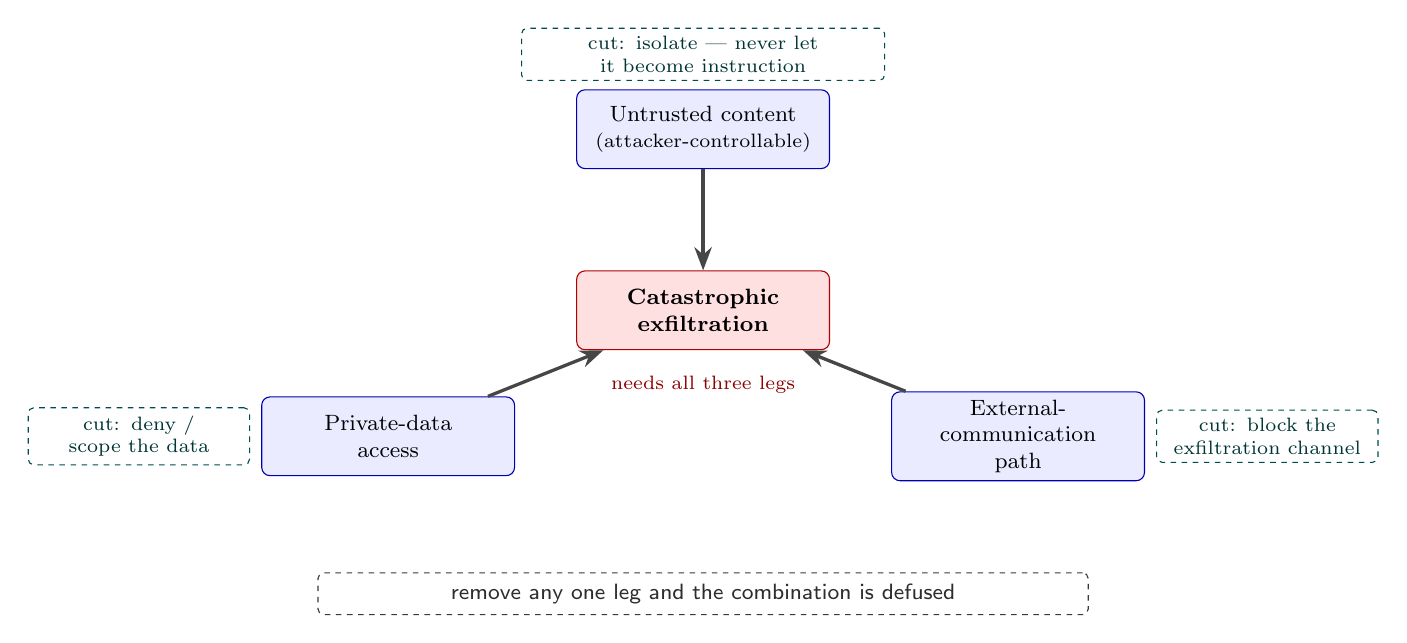
\begin{tikzpicture}[
  font=\sffamily,
  leg/.style={draw=blue!70!black, fill=blue!8, rounded corners=3pt, align=center,
    text width=3.0cm, minimum height=1.0cm, inner sep=3pt, font=\footnotesize},
  danger/.style={draw=red!70!black, fill=red!12, rounded corners=3pt, align=center,
    text width=3.0cm, minimum height=1.0cm, inner sep=3pt, font=\footnotesize\bfseries},
  edge/.style={-Stealth, very thick, draw=gray!55!black},
  cutnote/.style={draw=teal!60!black, dash pattern=on 2pt off 2pt, rounded corners=2pt,
    align=center, inner sep=3pt, font=\scriptsize, text=teal!40!black}
]

% three legs at the triangle corners
\node[leg] (untrusted) at (4,4.4) {Untrusted content\\{\scriptsize (attacker-controllable)}};
\node[leg] (private) at (0,0.5) {Private-data\\access};
\node[leg] (exfil) at (8,0.5) {External-communication\\path};

% the danger zone — only when all three are present
\node[danger] (cat) at (4,2.1) {Catastrophic\\exfiltration};
\node[font=\scriptsize, text=red!55!black] at (4,1.15) {needs all three legs};

% edges from each leg to the centre
\draw[edge] (untrusted) -- (cat);
\draw[edge] (private) -- (cat);
\draw[edge] (exfil) -- (cat);

% cut-here defense notes outside each leg
\node[cutnote, above=3pt of untrusted, text width=4.4cm] {cut: isolate --- never let it become instruction};
\node[cutnote, left=4pt of private, text width=2.6cm] {cut: deny / scope the data};
\node[cutnote, right=4pt of exfil, text width=2.6cm] {cut: block the exfiltration channel};

% footer
\node[draw=gray!45!black, dash pattern=on 2pt off 2pt, rounded corners=2pt, align=center,
  text width=9.5cm, inner sep=4pt, font=\sffamily\footnotesize, text=gray!35!black]
  at (4,-1.5) {remove any one leg and the combination is defused};

\end{tikzpicture}
\end{document}
